% Section I - Introduction. SOURCE OF TRUTH (the .md draft is superseded).
% Budget: ~380 for I-A+I-B (option B) or ~300 (option A); see word_budget_MLESP.md, advisor Q2. Cut here and in Section II first if long.

\subsection{Clinical motivation}
% REVIEW 2026-11-07 (space pass, blueprint Sec 9: cut from I and II first). No citation or claim dropped.
Major depressive disorder (MDD) is among the leading causes of disability worldwide \cite{ferrari2013}, yet its diagnosis still rests on clinical interviews and self-report scales of limited test-retest reliability \cite{lin2024,regier2013}. An objective physiological marker would help, and electroencephalography (EEG) is an attractive candidate: affordable, non-invasive, portable, and resolved on the millisecond scale \cite{simmatis2023}. Depression is increasingly understood to involve abnormal communication between large-scale brain networks \cite{kaiser2015}, and functional connectivity---the statistical dependence between signals at different sites, estimated with measures such as coherence, the phase-locking value or the phase lag index---captures that communication from scalp EEG. Deep networks learn from connectivity matrices directly, and a substantial literature applies them to separating people with MDD from healthy controls, many reporting accuracies above 90\% \cite{kaur2025}.

\subsection{The verification problem}
Accuracies of this magnitude would be clinically meaningful if they held. Whether they hold depends on something a reader usually cannot check: whether any information from the test data reached the model during training. This is data leakage, and in neuroimaging machine learning it has been shown to inflate reported performance substantially \cite{rosenblatt2024,yagis2021,lee2023}.

Recent reviews of EEG-based depression detection have examined how studies validate their models---holdout and cross-validation schemes, per-subject and leave-one-subject-out partitioning, and whether models were tested on independent datasets \cite{lin2024,lunaguevara2026}. That is the right question about the split. But a connectivity model does not consume raw EEG. It consumes a connectivity matrix, built through a chain of steps that each run before the split: recordings are epoched, connectivity is estimated, matrices are thresholded into graphs, values are normalized, and channels or frequency bands are selected. Each step can carry test information into training if it draws on data beyond the training fold, and most papers do not report the order of these steps, which leaves the question unanswerable from the paper alone. Fig.~\ref{fig:pipeline} contrasts a leakage-free ordering with a leaking one and marks the five points (L1--L5) at which test information can enter.

% REVIEW 2026-09-27 (E1): core-idea figure placed in the Introduction; IEEE floats it to the top of page 2.
\begin{figure*}[t]
\centering
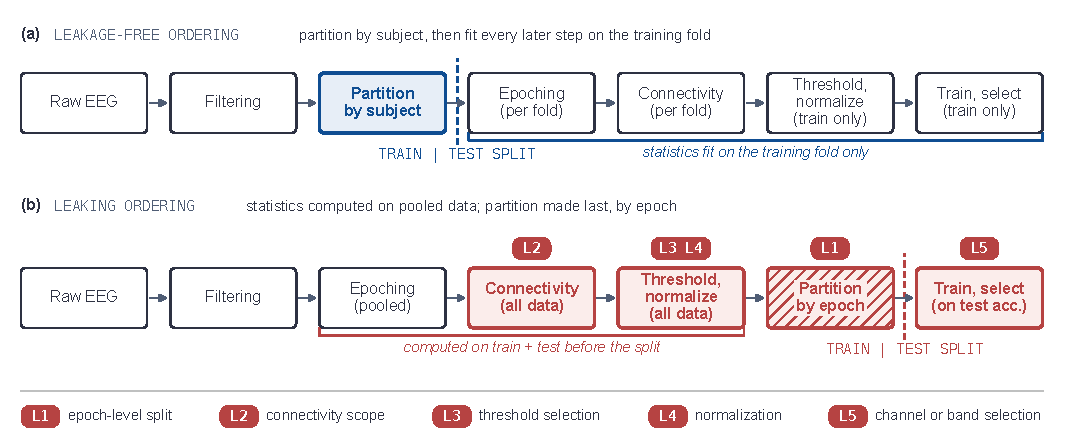
\includegraphics[width=0.74\textwidth]{figures/fig2_pipeline.pdf}
% REVIEW 2026-09-27 (C10)
\caption{The connectivity pipeline with leakage surfaces marked. (a) Leakage-free ordering: data are partitioned by subject before any statistic is computed, and every later step uses the training fold only. (b) Leaking ordering: connectivity (L2) and threshold or normalization statistics (L3, L4) are computed on pooled data, the partition is made by epoch so one subject can fall on both sides (L1), and channels or bands are chosen by test-set accuracy (L5). The dashed line marks the split. Red marks leakage points, hatching the epoch-level partition.}
\label{fig:pipeline}
\end{figure*}


Prior reviews audit how these studies split their data. This work audits what happens to the data before it is split. We searched PubMed, OpenAlex, Semantic Scholar and Google Scholar through September 2026 and found no review that audits connectivity-pipeline construction as a leakage surface in this literature; because that search was not itself conducted as a systematic review, we report it as the limit of our own searching rather than as a claim of priority.
% REVIEW 2026-11-07 (R2 W12): priority claim softened; the search was not systematic, so it cannot support one.

% REVIEW 2026-09-27 (C2): RQ1-RQ4 are used in Sections IV-VII but were never stated. Wording from blueprint RQ list.
We ask four questions. How completely do studies report each leakage surface (RQ1)? Can leakage risk be rated reliably from reported methods by independent raters (RQ2)? Is reported accuracy associated with the rating (RQ3)? And, as a secondary question, does reporting completeness change with publication year (RQ4)?
